\section{Evaluation}
\label{sec:eval}


We describe in detail our implementation method and evaluation procedure for
answering  our goals using the patent dataset. 

\subsection{Analysis Tools and Platform}


	\begin{itemize}
		% \squish
		\item We use IGraph library for all our graph analysis and metric
		calculation~\cite{igraph}. We use \texttt{matplotlib} library from Python to plot all our graphs.
		
		\item The configuration of our experimental desktop machine is RAM $32$ GB, $12$
		core with processor speed of $2.6$ GHz Intel® Xeon(R) CPU E5-2630 v2 and platform is Ubuntu $14.04$.
	\end{itemize}

\begin{table*}[t]
\centering
\begin{tabular}{clcl}
\hline
\multicolumn{1}{|l|}{\textbf{Rank}} & \multicolumn{1}{l|}{\textbf{Organization Name}}                  & \multicolumn{1}{l|}{\textbf{Rank}} & \multicolumn{1}{l|}{\textbf{Organization}}                     \\ \hline
\multicolumn{1}{|c|}{1}             & \multicolumn{1}{l|}{International Business Machines Corporation} & \multicolumn{1}{c|}{11}            & \multicolumn{1}{l|}{Hewlett Packard Company}                   \\ \hline
\multicolumn{1}{|c|}{2}             & \multicolumn{1}{l|}{Hitachi Ltd}                                 & \multicolumn{1}{c|}{12}            & \multicolumn{1}{l|}{Texas Instruments Incorporated}            \\ \hline
\multicolumn{1}{|c|}{3}             & \multicolumn{1}{l|}{Matsushita Electric Industrial Co Ltd,}      & \multicolumn{1}{c|}{13}            & \multicolumn{1}{l|}{Sony Corporation}                          \\ \hline
\multicolumn{1}{|c|}{4}             & \multicolumn{1}{l|}{Canon Kabushiki Kaisha,}                     & \multicolumn{1}{c|}{14}            & \multicolumn{1}{l|}{Intel Corporation}                         \\ \hline
\multicolumn{1}{|c|}{5}             & \multicolumn{1}{l|}{Motorola Inc,}                               & \multicolumn{1}{c|}{15}            & \multicolumn{1}{l|}{Micron Electric Co Ltd}                    \\ \hline
\multicolumn{1}{|c|}{6}             & \multicolumn{1}{l|}{Toshiba Corporation,}                        & \multicolumn{1}{c|}{16}            & \multicolumn{1}{l|}{Eastman Kodak Company}                     \\ \hline
\multicolumn{1}{|c|}{7}             & \multicolumn{1}{l|}{General Electric Company,}                   & \multicolumn{1}{c|}{17}            & \multicolumn{1}{l|}{Minnesota Mining \& Manufacturing Company} \\ \hline
\multicolumn{1}{|c|}{8}             & \multicolumn{1}{l|}{AT\&T Corp,}                                 & \multicolumn{1}{c|}{18}            & \multicolumn{1}{l|}{Microsoft Corporation}                     \\ \hline
\multicolumn{1}{|c|}{9}             & \multicolumn{1}{l|}{Fujitsu Limited,}                            & \multicolumn{1}{c|}{19}            & \multicolumn{1}{l|}{Samsung Electronics Co Ltd}                \\ \hline
\multicolumn{1}{|c|}{10}            & \multicolumn{1}{l|}{Xerox Corporation,}                          & \multicolumn{1}{c|}{20}            & \multicolumn{1}{l|}{NEC Corporation}                           \\ \hline                                                               
\end{tabular}
\caption{List of top 20 innovators for year 2013 as calculated by our proposed metrics.}
\label{lst:top20}
\end{table*}

\subsection{Evaluation Steps}
	\begin{itemize}
		% \squish
		\item {\em Evaluation Phase I - Collaborative Distance:} We calculate the 
		shortest path of each inventor w.r.t to Kia Silverbrook. We use three
		algorithms viz. Djikstra, Bellman-Ford, Johnson from IGraph to do this. We
		also analyze their scalability with respect to the invention network graph
		and compare their performance.
		\item {\em Social Network Behavior:} We compute the distribution of the 
		collaborative distance w.r.t. Kia Silverbrook for our network.
		\item {\em Evaluation Phase II - Degree centrality:} We use the in-built
		algorithm in IGraph to calculate degree centrality
		for each unique inventor and organization with respect to patents that cite his / her patent.
		\item {\em Data analysis and comparison:} We plot the graphs for the above
		generated data and analyze the relationship between the above two
		measurements. Then, we compare our ranking results for the most innovative organization
		with publicly available list such as Reuters list, to check if our ranking
		metric coincides with the results of other metrics.
	\end{itemize}



\subsection{Results}

\paragraph{Answer 1.}
We first calculate the total number of citations for each inventor from Graph G2. Using the collaboration distance calculated from G1, we plot a graph of distance (connectedness) vs. total number of citations (invention impact) of each inventor. 
Figure~\ref{fig:distance_citation} shows the relation of the distance from
Kia Silverbrook and the no. of total citations for an inventor. This graph gives a positive answer to Question 1: 
Yes, an inventor is more impactful because he is closely
connected to other impactful inventors in the patent social network.

\begin{figure}[t]
  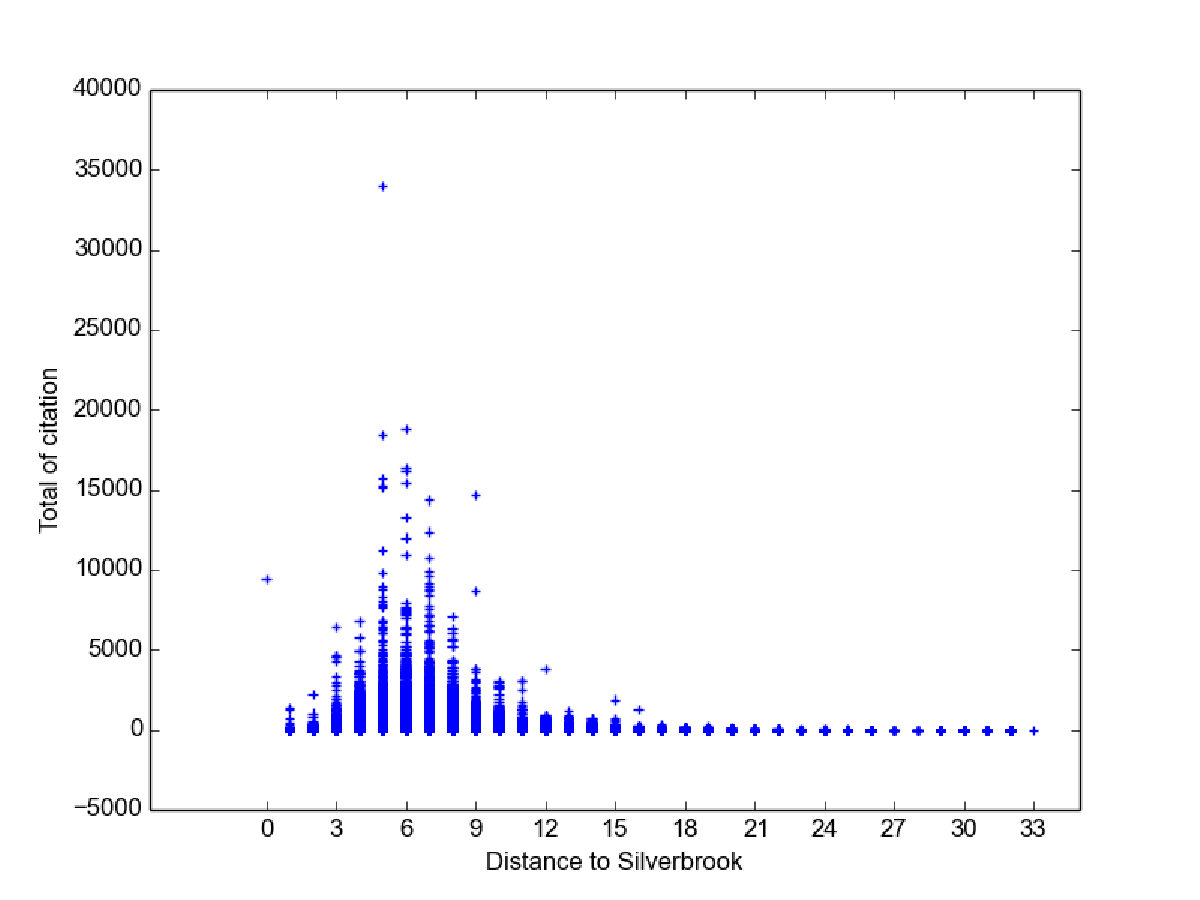
\includegraphics[scale=0.425]{figure/abc.pdf}
  \caption{ Relationship graph of no. of citations for all patents of an inventor (i.e., the cumulative degree centrality) and his distance from Kia Silverbrook}
\label{fig:distance_citation}
\end{figure}
\begin{figure}[t]
  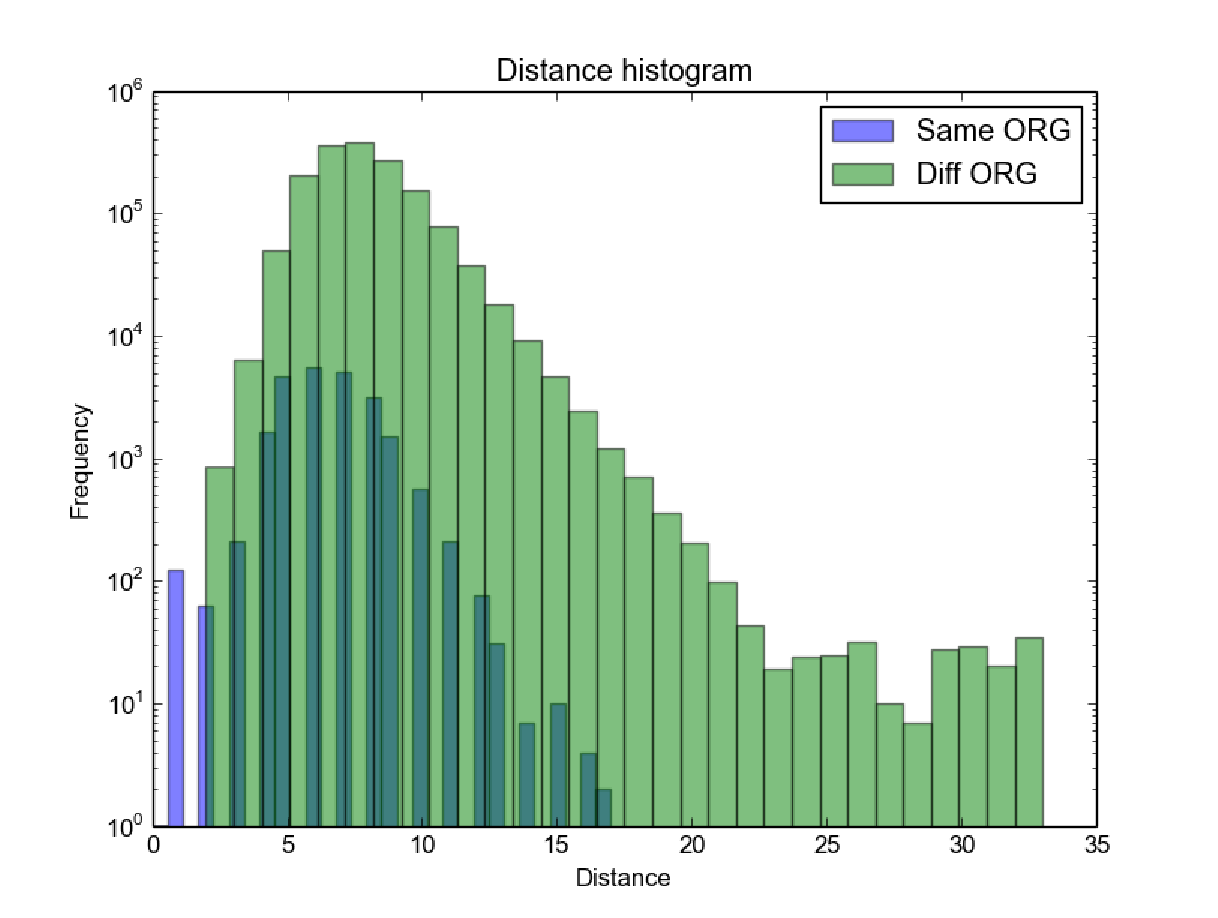
\includegraphics[scale=0.425]{figure/same_diff_org.pdf}
  \caption{ Relationship graph of organisation of an inventor and his distance from Kia Silverbrook}
\label{fig:same_diff}
\end{figure}

\paragraph{Answer 2.}
We divide each inventor into either same 
or different organization. An inventor belongs to 
 same organization category if he has patent with any of the organizations that are 
assignees for Kia Silverbrook's patents. All other inventors fall in the different
organization category. With this division, 
we plot a graph as shown in Figure~\ref{fig:same_diff}.
From the graph, we observe that inventors from same organization have
smaller collaborative distance which is expected. However, interesting observation is that
even many inventors from different organizations have smaller collaborative distance to Kia Silverbrook. 
This answers our Question 2:
Inventors are not only closely connected to an impactful
inventor in their own organization but also in other organizations.



\begin{table}[t]
\centering
\begin{tabular}{|l|c|c|}
\hline
\textbf{Organization}        & \multicolumn{1}{l|}{\textbf{24/7 Wall St}} & \multicolumn{1}{l|}{\textbf{SSL 3.0}} \\ \hline
IBM Corp                     & 1                                          & 1                                         \\ \hline
Samsung Electronics          & 2                                          & 19                                        \\ \hline
Canon K K                    & 3                                          & 4                                         \\ \hline
Sony Corp                    & 4                                          & 13                                        \\ \hline
Microsoft Corp               & 5                                          & 18                                        \\ \hline
\end{tabular}
\caption{Comparison of Rankings by 24/7 Wall St vs. SSL 3.0.}
\label{tab:validation}
\end{table}


\begin{table}[t]
\centering

		\begin{tabular}{| l | l |}
		\hline
		
		{Type} & {Count or Details} \\
		\hline
		\hline
		G1 Nodes & $3421276$ \\
		G1 Edges & $13153732$ \\
		G2 Nodes & $10842560$ \\
		G2 Edges & $53527305$ \\
		G1 Source Node & Kia Silverbrook \\
		Infinite dist. within Org & $6217$\\
		Infinite dist. outside Org& $1817586$ \\
		Patents with zero citations & $1349956$ \\
		\hline
	\end{tabular}		
	\caption { Details of the co-authorship graph.}
	\label{tab:model}
\end{table}	

\begin{table}[t]
\centering

	\begin{tabular}{| l | l |}
		\hline
		{Algorithm} & {Time (sec)} \\
		\hline
		\hline
		Bellman-Ford & $0.80$ \\
		Dijkstra & $1.28$ \\
		Johnson & $1.29$ \\
		\hline
	\end{tabular}
	\caption { Performance of the three shortest path algorithms}
	\label{tab:algos}
\end{table}		

\begin{figure}[t]
  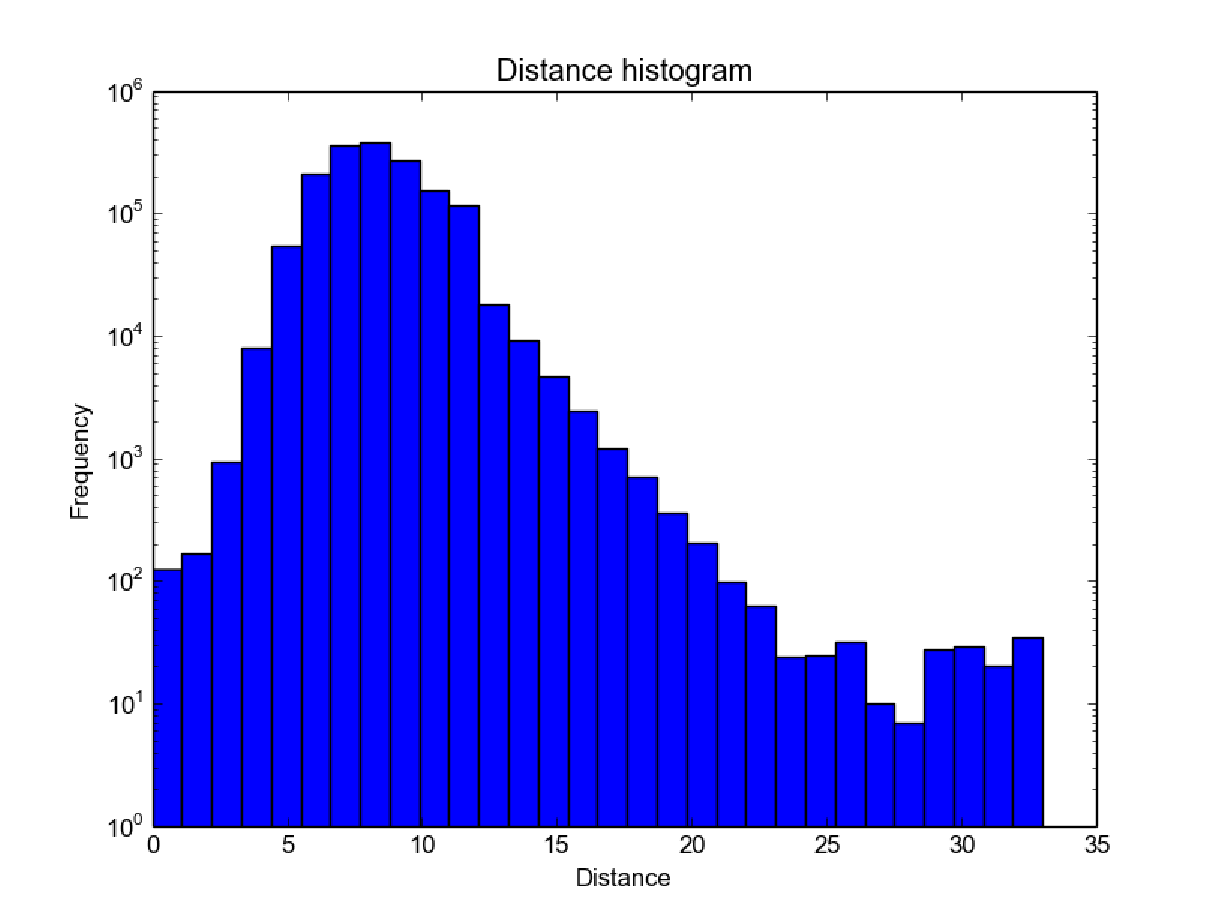
\includegraphics[scale=0.425]{figure/silver_brook_distance.pdf}
  \caption{ Graph shows the frequency of nodes on Y-axis and the distance from
Kia Silverbrook on X-axis }
\label{fig:distance}
\end{figure}

\begin{figure}
  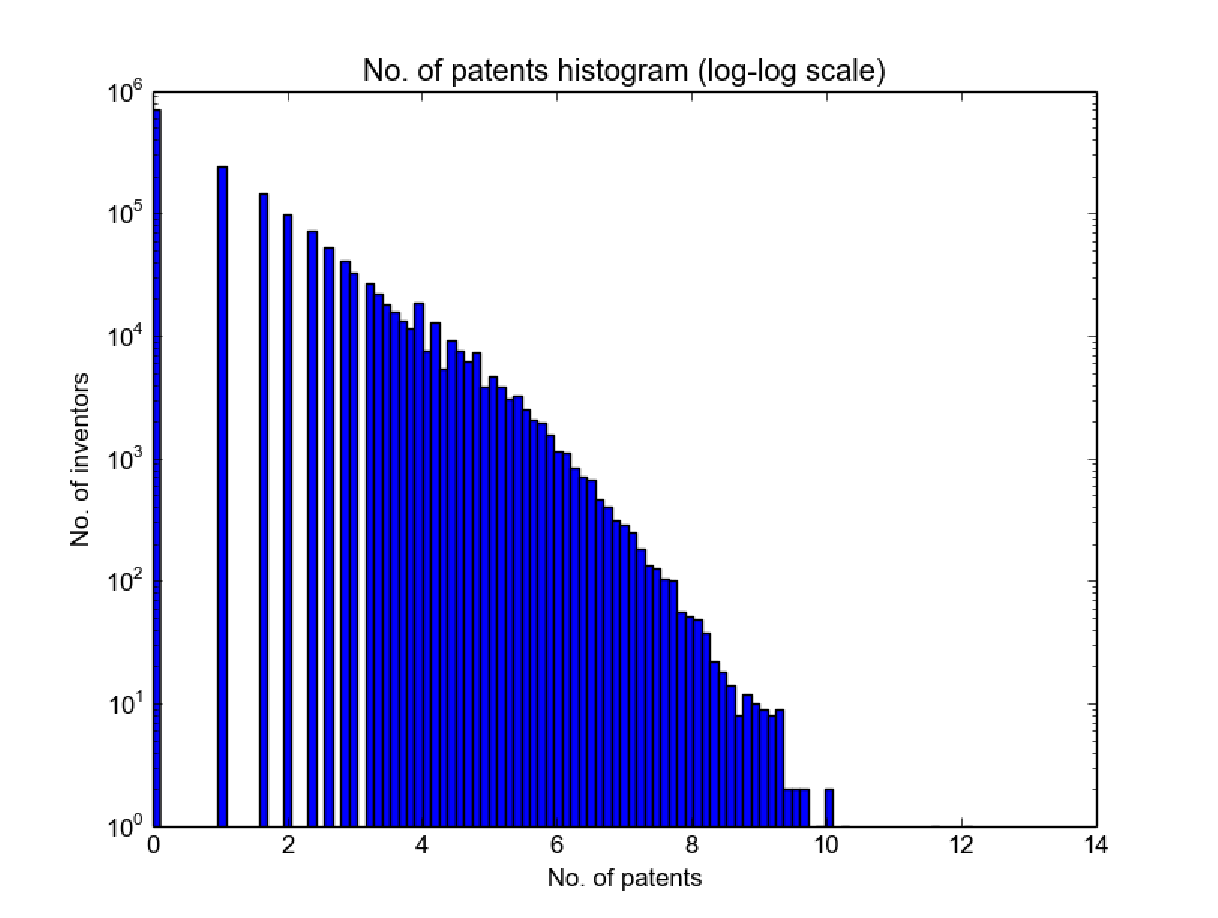
\includegraphics[scale=0.425]{figure/silver_log_log.pdf}
  \caption{ Log-log scale graph of no. of patents on Y-axis and the no.of inventors on X-axis}
\label{fig:patent}	
\end{figure}

\begin{figure}[t]
  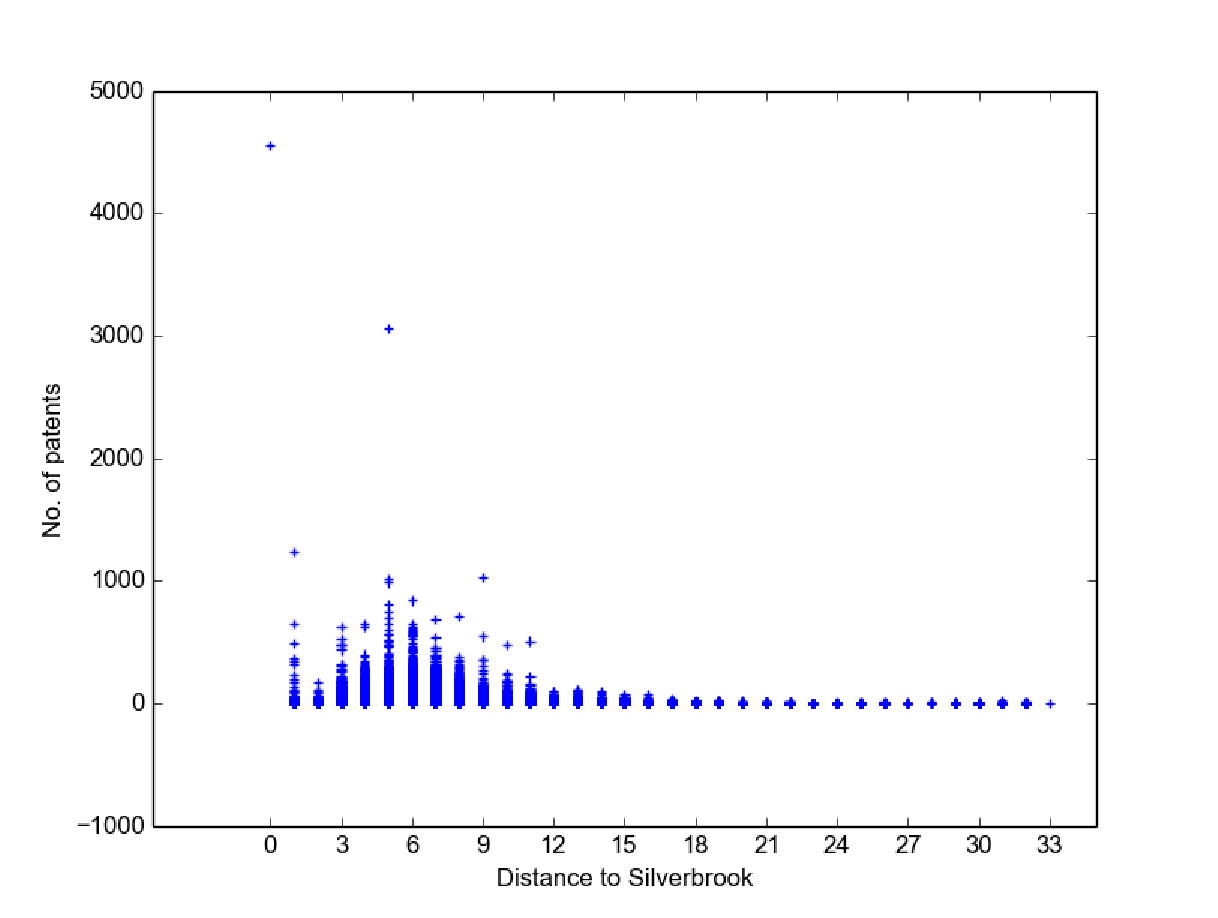
\includegraphics[scale=0.425]{figure/distance_patents.pdf}
  \caption{Relationship graph of no. of patents of an inventor and his distance from Kia Silverbrook}
\label{fig:distance_patent}
\end{figure}

\paragraph{Answer 3.}
We calculate the total number of citations for all patents assigned to a particular organization using graph G2. We rank the organizations based on this metric of total number of citations. Table~\ref{lst:top20} shows the top 20 organisations that are leading the innovation industry via impactful inventions in last four decades, as per our metric. 
This answers our Q3. 

\paragraph{Validating Answer 3.}
To validate the fairness of our proposed metrics, we cross-check our rankings
with public ally available rankings for the year 2013 by 24/7 Wall Street and
Reuters. These two lists are representatives of quantity and quality
respectively.  24/7 Wall Street report is purely based on number of patents
granted to an organization till that year.  On the other hand, Reuters
consider both quantitative as well as qualitative factors with respect to
time. Specifically, the factors such as volume of patents filed in last five
years, success ratio of filed patents, global contributions apart from US
patents, and citation impact of invention in last five years~\cite{reuters-method}.

Table~\ref{tab:validation} shows the top 5 innovative organizations in 2013 as
reported by 24/7 Wall Street and the corresponding rankings as per our
proposed metrics. We report that all of these 5 organizations occur in top 20
list as per our metrics (See Table~\ref{lst:top20} for the complete list).
This validates that our metric fairly succeeds in covering the quantitative
aspects of innovation.

We also compare our rankings to the list of top 100 innovators by Thomas
Reuters. Their report only states the top 100 innovators and does not give any
rankings. Thus, we only compare the percentage of organizations that fall in
top 100 in both Reuters are well as our rankings. On analysis, we find that
this intersection size is 41\%, which validates that our metric fairly
succeeds in covering the qualitative aspects of innovation.


\subsection{Miscellaneous Results}

Apart from answering the research questions, we also report the statistics about the inventor network that we collected during our study:

	\begin{itemize}
	% \squish
	\item {\em Graph Details.}
	Table~\ref{tab:model} gives the details
	about Graph G1 in terms of its total number of inventors (nodes), patents (edges), and the
	source node of the graph. We choose Kia Silverbrook as our source node as he is one
	of the top and popular inventors in the patent dataset with maximum number of
	patents. We calculate the shortest path of all other nodes from Kia Silverbrook.
	Our analysis shows that there are $6217$ inventors within Kia Silverbrook's organizations 
	and $1817586$ inventors out side his organization that have infinite collaborative distance (not connected).
	Similarly, for Graph G2, Table~\ref{tab:model} gives the total number of patents (nodes), citations (edges), island patents (i.e., patents with zero citations).

	\item {\em Performance Comparison.}
	We run three algorithms particularly Djikstra shortest path algorithm,
	Bellman-ford and Johnson available in IGraph tool on our Graph G1.
	Table~\ref{tab:algos} shows the execution time for each of the three shortest
	path algorithms  when run on our graph G1. We observe that Djikstra's
	algorithm takes $1.28$ seconds, Bellman-ford takes $0.80$ seconds and Johnson
	algorithm takes $1.29$ seconds to run on our experimental setup.
	
	\item {\em Collaborative Distance Characteristics.}
	Figure~\ref{fig:distance} shows the result for the total number of inventors
	having the same distance from Kia Silverbrook. Figure~\ref{fig:patent} shows the log-log graph of the total no.of patents to total no.of inventors. 

	\item{\em Distribution of Quantitative Innovation Impact.}
	Figure~\ref{fig:distance_patent} shows the relation of the distance from
	Kia Silverbrook and the no. of patents for an inventor. 
	\end{itemize}
